\section{Структуры данных в линейных решениях}

\tikzset{
    queue element/.style={
        draw,very thin,rounded corners,
        fill=yellow!30,
        minimum width=1cm,minimum height=.5cm,
        font=\footnotesize
    }
}

\subsection{Стек и его применения в задачах}

\begin{definition}
    \textit{Стек} --- структура данных, представляющая из себя упорядоченный набор элементов, в которой добавление новых \mbox{элементов} и удаление существующих производится с одного конца, называемого \textit{\mbox{вершиной} стека}.
\end{definition}

\begin{center}
    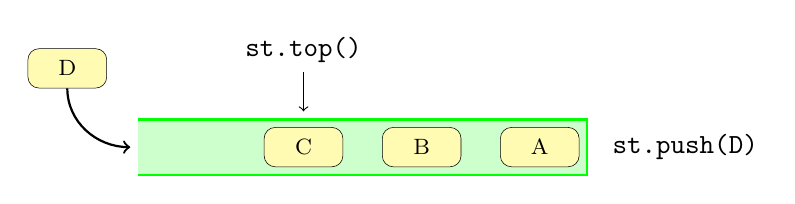
\begin{tikzpicture}
        \fill[green!20] (5.1,.35) rectangle (-.6,-.35);
        \draw[green,thick] (-.6,.35) -- (5.1,.35) |- (-.6,-.35);
        \foreach \i/\name in {1/C,2/B,3/A}
            \node[queue element] (\name) at (1.5*\i,0) {\name};
        \draw[<-] ([yshift=.2cm]C.north) -- ++ (0,.5) node[above] {\texttt{st.top()}};
        \path (5.3,0) node[right] {\texttt{st.push(D)}};
        \node[queue element] (D) at (-1.5,1) {D};
        \draw[->, thick] (D.south) to[out=-90,in=180] (-.7,0);
    \end{tikzpicture}
    \medskip
    
    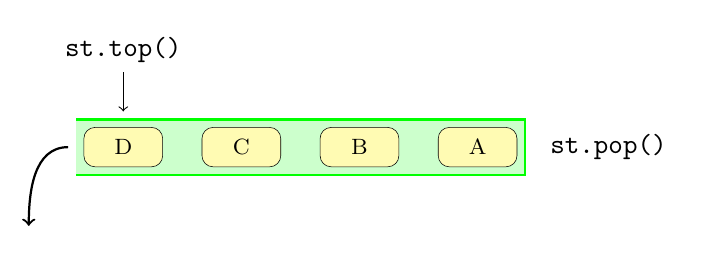
\begin{tikzpicture}
        \fill[green!20] (5.1,.35) rectangle (-.6,-.35);
        \draw[green,thick] (-.6,.35) -- (5.1,.35) |- (-.6,-.35);
        \foreach \i/\name in {0/D,1/C,2/B,3/A}
            \node[queue element] (\name) at (1.5*\i,0) {\name};
        \draw[<-] ([yshift=.2cm]D.north) -- ++ (0,.5) node[above] {\texttt{st.top()}};
        \draw[->, thick] (-.7,0) to[out=180,in=90] ++ (-.5,-1);
        \path (5.3,0) node[right] {\texttt{st.pop()}};
    \end{tikzpicture}
\end{center}

\begin{problem}
    Для каждого элемента массива $\{a_1, a_2, \ldots, a_n\}$ найти ближайший справа элемент, меньший него.
\end{problem}

Если решать <<в лоб>>, то максимальное количество операций равно 
\[(n - 1) + (n - 2) + \ldots + 1 = \frac{n(n - 1)}{2} = O(n^2),\]
достигается при отсортированном по возрастанию массиве.

Для линейного решения предварительно добавим в массив граничные элементы $a_0 \vcentcolon = -\infty$, $a_{n + 1} \vcentcolon = -\infty$ и создадим стек, положив в него индекс $0$. Будем идти по массиву $\{a_1, a_2, \ldots, a_{n + 1}\}$ слева направо и \mbox{сравнивать} каждый элемент массива $a_i$ с элементом массива, доступным по \mbox{верхнему} индексу стека. Пока $a_i$ меньше верхнего элемента стека, будем удалять этот верхний элемент и записывать $i$ в качестве ответа для него. Затем добавим $i$ в стек.

Обоснуем корректность этого алгоритма. Сначала заметим, что стек никогда не остаётся пустым и каждый элемент хоть раз будет в него добавлен (в силу того, что $a_0 = -\infty$). Также, для каждого элемента будет записан ответ (в силу того, что $a_{n + 1} = -\infty$). Записанный ответ является правильным, т.\,к. для каждого числа записывается первое, меньшее него.

\begin{minted}[linenos, mathescape]{cpp}
vector<int> ans(n + 2);
stack<int> st; st.push(0);
for (int i = 1; i < n + 2; ++i)
{
    while (a[st.top()] > a[i])
        ans[st.top()] = i, st.pop();
    st.push(i);
}
\end{minted}

\begin{problem}[Гистограмма]
    Дан массив $\{h_1, h_2, \ldots, h_n\}$, представленный в~виде гистограммы. Требуется найти наибольшую площадь прямоугольника, вписанного в эту гистограмму.
\end{problem}

Заметим, что искомый прямоугольник имеет высоту, совпадающую с~высотой одного из столбцов. Действительно, если это не так, то можно увеличить его площадь, подняв до ближайшего столбца. Будем перебирать высоты прямоугольника и для каждой из них находить левую и правую границы с помощью предыдущей задачи. Для каждого столбца это можно сделать заранее и ответами заполнить \mbox{массивы} $\{l_1, l_2, \ldots, l_n\}$ и $\{r_1, r_2, \ldots, r_n\}$. Тогда площадь прямоугольника высотой $h_i$ равна $S_i \hm = h_i(r_i - l_i - 1)$.

\begin{problem}
    В массиве $\{\rlap{$\overbracket[.2mm]{\phantom{a_1, a_2, \ldots, a_k}}$}a_1, \underbracket[.2mm]{a_2, \ldots, a_k, a_{k + 1}}, \ldots, a_n\}$ найти минимум в скользящем окне шириной $k$.
\end{problem}

Решим задачу о нахождении ближайшего справа элемента меньше \mbox{текущего} и ответы запишем в массив $\{b_0, b_1, \ldots, b_{n + 1}\}$. Положим \mbox{$i = 1$} (указывает на первый элемент первого окна), а затем будем делать \mbox{замену} $i \mapsto b_i$, пока $b_i$ не выходит за границы окна. В конце $i$ будет указывать на~минимальный элемент в этом окне, т.\,к. $a_i$ меньше всех \mbox{элементов} \mbox{окна}, стоящих левее него, а первый элемент правее и \mbox{меньше} него уже не~\mbox{попадает} в окно. При переходе к новому окну если текущее значение $i$ в него не попадает, то ставим $i$ на позицию первого элемента нового окна.

Данный алгоритм работает за линейное время, т.\,к. $b_i > i$ для каждого индекса $i$. Таким образом, на каждом шаге мы двигаемся вперёд по \mbox{массиву} хотя бы на $1$. Всего элементов в массиве $n$, значит, шагов алгоритма не более $n$. Худший случай --- отсортированный по убыванию массив, на котором каждый раз мы двигаемся ровно на $1$ шаг.

\begin{minted}[linenos, mathescape]{cpp}
int i = 1;
vector<int> ans(n - k + 2);
for (int j = 1; j <= n - k + 1; ++j)
{
    if (i < j) i = j;
    while (b[i] < j + k) i = b[i];
    ans[j] = i;
}
\end{minted}

\begin{definition}
    Скобочная последовательность $s$ называется \textit{правильной}, если $s$ пуста или $s = (s^\prime)$, где $s^\prime$ --- правильная скобочная последовательность, или $s = s_1s_2$, где $s_1$ и $s_2$ --- правильные скобочные последовательности.
\end{definition}

\begin{problem}
    По данной скобочной последовательности проверить, является ли она правильной.
\end{problem}

Заведём стек, в который изначально добавим первый символ данной последовательности. Далее будем идти по символам этой строки и если встретили закрывающую скобку, то сверху стека должна быть открывающая (соответствующая этой закрывающей). Тогда удалим этот элемент стека, а иначе добавим новый символ в стек. Если по окончании стек пуст, то наша скобочная последовательность правильная, иначе --- нет.

\subsection{Очередь}

\begin{definition}
    \textit{Очередь} --- это структура данных, добавление и удаление элементов в которой происходит так, что первым из очереди удаляется элемент, который был помещен туда первым. У очереди имеется \textit{хвост}, куда добавляются элементы, и \textit{голова}, откуда они удаляются. 
\end{definition}

\begin{center}
    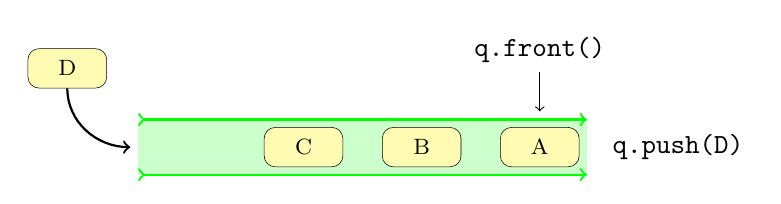
\begin{tikzpicture}
        \fill[green!20] (5.1,.35) rectangle (-.6,-.35);
        \draw[green,thick,>->] (-.6,.35) -- (5.1,.35);
        \draw[green,thick,>->] (-.6,-.35) -- (5.1,-.35);
        \foreach \i/\name in {1/C,2/B,3/A}
            \node[queue element] (\name) at (1.5*\i,0) {\name};
        \draw[<-] ([yshift=.2cm]A.north) -- ++ (0,.5) node[above] {\texttt{q.front()}};
        \path (5.3,0) node[right] {\texttt{q.push(D)}};
        \node[queue element] (D) at (-1.5,1) {D};
        \draw[->, thick] (D.south) to[out=-90,in=180] (-.7,0);
    \end{tikzpicture}

    \hspace{1cm}
    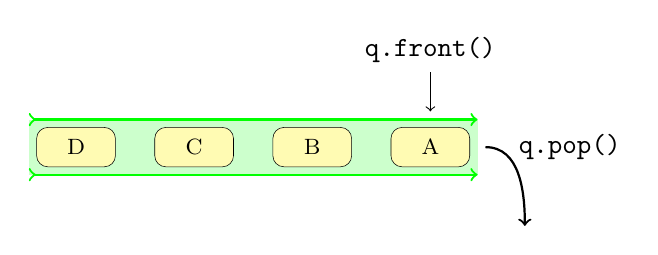
\begin{tikzpicture}
        \fill[green!20] (5.1,.35) rectangle (-.6,-.35);
        \draw[green,thick,>->] (-.6,.35) -- (5.1,.35);
        \draw[green,thick,>->] (-.6,-.35) -- (5.1,-.35);
        \foreach \i/\name in {0/D,1/C,2/B,3/A}
            \node[queue element] (\name) at (1.5*\i,0) {\name};
        \draw[<-] ([yshift=.2cm]A.north) -- ++ (0,.5) node[above] {\texttt{q.front()}};
        \draw[->, thick] (5.2,0) to[out=0,in=90] ++ (.5,-1);
        \path (5.5,0) node[right] {\texttt{q.pop()}};
    \end{tikzpicture}
\end{center}

Одним из основных применений очереди --- является реализация поиска в ширину, про это будет рассказано больше.

\subsection{Дек и второе решение задачи о минимуме в окне}

\begin{definition}
    \textit{Дек} --- структура данных, представляющая из себя \mbox{список} элементов, в которой добавление новых элементов и удаление \mbox{существующих} производится с обоих концов. 
\end{definition}

\begin{center}
    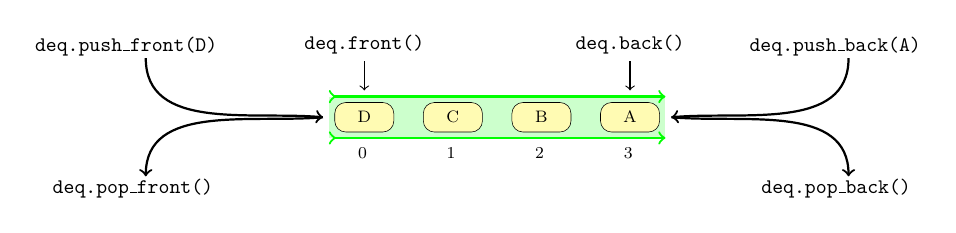
\begin{tikzpicture}[scale=.75, every node/.style={scale=.75}]
        \fill[green!20] (5.1,.35) rectangle (-.6,-.35);
        \draw[green,thick,>->] (-.6,.35) -- (5.1,.35);
        \draw[green,thick,>->] (-.6,-.35) -- (5.1,-.35);
        \foreach \i/\name in {0/D,1/C,2/B,3/A}
            \node[queue element] (\name) at (1.5*\i,0) {\name};
        \foreach \i in {0,1,2,3}
            \path (1.5*\i-.23,-.6) node [right] {\footnotesize $\i$};
        \draw[<-] ([yshift=.2cm]A.north) -- ++ (0,.5) node[above] {\texttt{deq.back()}};
        \draw[<-] ([yshift=.2cm]D.north) -- ++ (0,.5) node[above] {\texttt{deq.front()}};
        \path (-5.4,-1.2) node[right] {\texttt{deq.pop$\_$front()}};
        \path (-5.7,1.2) node[right] {\texttt{deq.push$\_$front(D)}};
        \draw[->, thick] (-.7,0) to[out=185,in=90] ++ (-3,-1);
        \draw[<-, thick] (-.7,0) to[out=175,in=-90] ++ (-3,1);
        \draw[->, thick] (5.2,0) to[out=-5,in=90] ++ (3,-1);
        \draw[<-, thick] (5.2,0) to[out=5,in=-90] ++ (3,1);
        \path (6.6,-1.2) node[right] {\texttt{deq.pop$\_$back()}};
        \path (6.4,1.2) node[right] {\texttt{deq.push$\_$back(A)}};
    \end{tikzpicture}
\end{center}

Отметим, что на дек бывает удобно смотреть как на двустороннюю очередь с индексацией.

Предложим другое решение задачи о поиске минимума в \mbox{скользящем} окне в массиве $\{a_0, a_1, \ldots, a_{n - 1}\}$ (в этот раз нам удобнее вести индексацию с $0$). Назовём элемент \textit{перспективным} для~данного окна, если в этом окне нет элементов правее и не больше него. Это условие необходимо для того, чтобы какой-то элемент был \mbox{минимумом} в~данном окне, поэтому этот минимум принадлежит множеству перспективных элементов. Заметим, что последовательность перспективных элементов неубывающая, а потому минимумом является первый элемент этой последовательности. Искать его будем так: заведём дек и сначала положим в него $0$ (\mbox{указывает} на первый элемент первого окна), а каждый следующий элемент будем добавлять, предварительно удалив из дека все элементы, большие этого следующего. Для перехода к новому окну удалим из дека первый элемент предыдущего окна, если он там есть (при~этом он всегда будет в начале дека), и добавим последний элемент нового указанным способом.

\begin{minted}[linenos, mathescape]{cpp}
deque<int> deq;
for (int i = 0; i < n; ++i)
{
    if (i >= k && deq.front() == i - k) deq.pop_front();
    while (deq.size() && a[deq.back()] >= a[i]) deq.pop_back();
    deq.push_back(i);
    if (i >= k - 1)
        ans.push_back(deq.front());
}
\end{minted}

Для каждого из вышеперечисленных контейнеров определены методы \texttt{.size()}, возвращающий количество его элементов, и \texttt{.empty()}, проверяющий его на пустоту.
